\begin{name}
	{Biên soạn \& Phản biện: Nhóm 2}
	{Sở GD \& ĐT Sơn La (Lần 2)}
\end{name}
\Opensolutionfile{ansbook}[ans/ansb\currfilebase]
\caulc
\Opensolutionfile{ans}[ans/ans\currfilebase-Phan-I]
\begin{ex}%[Dự án 3191BS-VN-MT-15]%[2-KS-21-SoSonLa-L2-2026,VM038]%[1D5H1-3] 
	Doanh thu bán hàng trong $20$ ngày được lựa chọn ngẫu nhiên của một cửa hàng được ghi lại ở bảng sau (đơn vị: triệu đồng):\\
	\centerline{\begin{tabular}{|c|c|c|c|c|c|}
		\hline
		Doanh thu & $[5;7)$ & $[7;9)$ & $[9;11)$ & $[11;13)$ & $[13;15)$\\
		\hline
		Số ngày & 2 & 7 & 7 & 3 & 1\\
		\hline
	\end{tabular}}\\
	Số trung bình của mẫu số liệu trên thuộc nhóm nào trong các nhóm dưới đây?
	\choice
		{$[7;9)$}
		{\True $[9;11)$}
		{$[11;13)$}
		{$[13;15)$}
	\loigiai{
		\\
		Bảng giá trị đại diện là\\
		\centerline{\begin{tabular}{|c|c|c|c|c|c|}
			\hline
			Giá trị đại diện & $6$ & $8$ & $10$ & $12$ & $14$\\
			\hline
			Số ngày & 2 & 7 & 7 & 3 & 1\\
			\hline
		\end{tabular}}\\
		Số trung bình của mẫu số liệu là
		\[\overline{x}=\dfrac{6\cdot2+8\cdot7+10\cdot7+12\cdot3+14\cdot1}{20}=\dfrac{188}{20}=9{,}4.\]}
\end{ex}

\begin{ex}%[Dự án 5DE4BE-VN-MT-15]%[2-KS-21-SoSonLa-L2-2026,VM038]%[1H8H7-3] 
	Cho hình chóp đều $S.ABCD$ có cạnh đáy bằng $a\sqrt{2}$, cạnh bên bằng $2a$. Thể tích khối chóp $S.ABCD$ là
	\choice
		{$\dfrac{4a^3}{3}$}
		{$\dfrac{a^3}{3}$}
		{\True $\dfrac{2a^3\sqrt{3}}{3}$}
		{$\dfrac{2a^3}{3}$}
	\loigiai{
		\begin{center}
			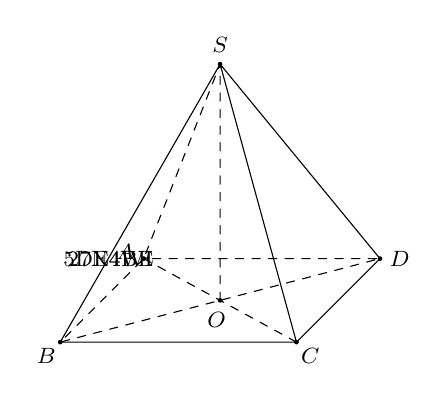
\begin{tikzpicture}[scale=1,>=stealth, font=\footnotesize, line join=round, line cap=round]
    %hidden: VM005
				%hidden: VM038
				\path
					(0,0) coordinate (A)
					++(-135:1.5) coordinate (B)
					++(0:3) coordinate (C)
					(barycentric cs:A=1,C=1,B=-1)coordinate(D)
					(barycentric cs:A=1,C=1)coordinate(O)
					(O)+(90:3) coordinate (S)
					;
				\draw[dashed] (O)--(S)--(A)--(B)--(D) (C)--(A)--(D);
				\draw (C)--(S)--(B)--(C)--(D)--(S);
				\foreach \p/\g in{A/160,B/-135,C/-45,D/0,O/-100,S/90}
				\fill(\p)circle(.03)node[shift={(\g:.25)},scale=1]{$\p$};
				\node at (0,0){\href{27N4WI}{\tiny \phantom{27N4WI}}};
    \node at (0,0){\href{5DE4BE}{\tiny \phantom{5DE4BE}}};
			\end{tikzpicture}
		\end{center}
		Diện tích đáy $ABCD$ là $S=\left( a\sqrt{2}\right)^2=2a^2$.\\
		Gọi $O$ là tâm hình vuông $ABCD$. Khi đó $SO\perp (ABCD)$ và $OA=\dfrac{1}{2}AC=\dfrac{a\sqrt{2}\cdot\sqrt{2}}{2}=a$.\\
		Suy ra $SO=\sqrt{SA^2-OA^2}=\sqrt{(2a)^2-a^2}=a\sqrt{3}$.\\
		Thể tích khối chóp đều $S.ABCD$ là
		\[V=\dfrac{1}{3}S\cdot SO=\dfrac{1}{3}\cdot2a^2\cdot a\sqrt{3}=\dfrac{2a^3\sqrt{3}}{3}.\]}
\end{ex}

\begin{ex}%[Dự án ZRWTK9-VN-MT-15]%[2-KS-21-SoSonLa-L2-2026,VM038]%[1H8H2-2] 
	Cho hình chóp $S.ABCD$ có đáy là hình bình hành tâm $O$, $SA=SC$, $SB=SD$. Trong các khẳng định sau khẳng định nào đúng?
	\choice
		{\True $SO\perp (ABCD)$}
		{$SC\perp (ABCD)$}
		{$SB\perp (ABCD)$}
		{$SA\perp (ABCD)$}
	\loigiai{
		\begin{center}
			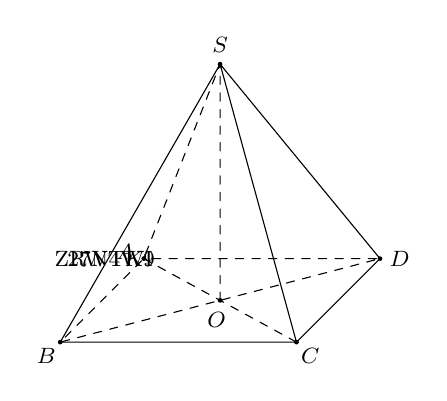
\begin{tikzpicture}[scale=1,>=stealth, font=\footnotesize, line join=round, line cap=round]
    %hidden: VM005
				\path
					(0,0) coordinate (A)
					++(-135:1.5) coordinate (B)
					++(0:3) coordinate (C)
					(barycentric cs:A=1,C=1,B=-1)coordinate(D)
					(barycentric cs:A=1,C=1)coordinate(O)
					(O)+(90:3) coordinate (S)
					;
				\draw[dashed] (O)--(S)--(A)--(B)--(D) (C)--(A)--(D);
				\draw (C)--(S)--(B)--(C)--(D)--(S);
				\foreach \p/\g in{A/160,B/-135,C/-45,D/0,O/-100,S/90}
				\fill(\p)circle(.03)node[shift={(\g:.25)},scale=1]{$\p$};
				\node at (0,0){\href{27N4WI}{\tiny \phantom{27N4WI}}};
    \node at (0,0){\href{ZRWTK9}{\tiny \phantom{ZRWTK9}}};
			\end{tikzpicture}
		\end{center}
		Vì $ABCD$ là hình bình hành tâm $O$ nên $OA=OC$, $OB=OD$.\\
		Theo giả thiết $SA=SC$, $SB=SD$ nên $SO$ là đường trung trực của các đoạn thẳng $AC$ và $BD$.\\
		Suy ra $SO\perp AC$ và $SO\perp BD$.\\
		Do đó $SO\perp(ABCD)$.\\
		Qua $S$ có duy nhất một đường thẳng vuông góc với mặt phẳng $(ABCD)$ nên các khẳng định $SC\perp(ABCD)$, $SB\perp(ABCD)$, $SA\perp(ABCD)$ là sai.
	}
\end{ex}

\begin{ex}%[Dự án 3QO9CH-VN-MT-15]%[2-KS-21-SoSonLa-L2-2026,VM038]%[2H5N1-2] 
	Trong không gian $Oxyz$, vectơ nào sau đây là một vectơ pháp tuyến của mặt phẳng $(P)\colon 2x-y+z+3=0$?
	\choice
		{\True $\overrightarrow n_1=(2;-1;1)$}
		{$\overrightarrow n_3=(2;-1;3)$}
		{$\overrightarrow n_2=(2;1;1)$}
		{$\overrightarrow n_4=(-1;1;3)$}
	\loigiai{
		Mặt phẳng $(P)\colon 2x-y+z+3=0$ có một vectơ pháp tuyến là $\overrightarrow n=(2;-1;1)$.}
\end{ex}

\begin{ex}%[Dự án A2MWC4-VN-MT-15]%[2-KS-21-SoSonLa-L2-2026,VM038]%[2D4N2-1] 
	Cho $\displaystyle\int\limits_0^1 f(x)\mathrm{\,d} x=1$ và $\displaystyle\int\limits_0^2 f(x)\mathrm{\,d} x=-4$. Tích phân $\displaystyle\int\limits_1^2 f(x)\mathrm{\,d} x$ bằng
	\choice
		{$3$}
		{$5$}
		{$-3$}
		{\True $-5$}
	\loigiai{
		Ta có
		$\displaystyle\int\limits_1^2 f(x)\mathrm{\,d} x=\displaystyle\int\limits_0^2 f(x)\mathrm{\,d} x-\displaystyle\int\limits_0^1 f(x)\mathrm{\,d} x=-4-1=-5$.
	}
\end{ex}

\begin{ex}%[Dự án 26A0Y2-VN-MT-15]%[2-KS-21-SoSonLa-L2-2026,VM038]%[2D1N2-2] 
	\immini[thm]{Cho hàm số $y=f(x)$ có đồ thị như hình vẽ. Điểm cực tiểu của hàm số đó là
		\choice[2]
			{$x=-2$}
			{\True $x=2$}
			{$x=0$}
			{$y=-2$}}
			{
			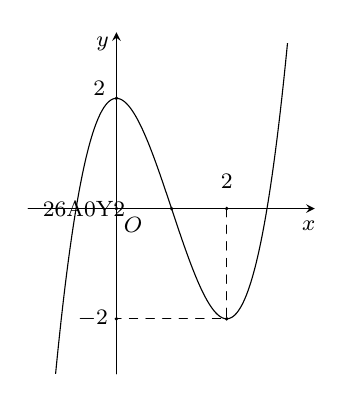
\begin{tikzpicture}[scale=0.7,>=stealth, font=\footnotesize, line join=round, line cap=round]
    %hidden: VM005
				\draw[->] (-1.6,0)--(3.6,0)node[shift={(-110:.23)}]{$x$};
				\draw[->] (0,-3)--(0,3.2)node[shift={(220:.23)}]{$y$};
				\path(0,0)node[shift={(-45:.3)}]{$O$} (0,2)node[shift={(150:.25)}]{$2$};
				\clip (-1.5,-3) rectangle (3.5,3);
				\draw[smooth,samples=300,domain=-2:3.5] plot(\x,{(\x)^3-3*(\x)^2+2});
				\draw[dashed] 
					(2,0) node[shift={(90:.35)}]{$2$}|-(0,-2)node[shift={(180:.3)}]{$-2$}
					;
				\foreach \x/\y in{0/0,2/-2,1/0,2/0,0/2,0/-2}
				\fill (\x,\y) circle (1pt);
    \node at (0,0){\href{26A0Y2}{\tiny \phantom{26A0Y2}}};
			\end{tikzpicture}
			}
	\loigiai{
		Từ đồ thị, điểm cực tiểu của hàm số là $x=2$.}
\end{ex}

\begin{ex}%[Dự án XADI0Z-VN-MT-15]%[2-KS-21-SoSonLa-L2-2026,VM038]%[2D4N1-3] 
	Họ tất cả các nguyên hàm của hàm số $f(x)=\sin x$ là
	\choice
		{$-\sin x+C$}
		{$\sin x+C$}
		{\True $-\cos x+C$}
		{$\cos x+C$}
	\loigiai{
		Ta có $\displaystyle\int\sin x\mathrm{\,d}x=-\cos x+C$.
	}
\end{ex}

\begin{ex}%[Dự án 3M9GSU-VN-MT-15]%[2-KS-21-SoSonLa-L2-2026,VM038]%[2H5N3-2] 
	Trong không gian $Oxyz$, cho mặt cầu $(S)\colon (x-2)^2+(y+1)^2+(z-3)^2=4$. Tâm của $(S)$ có tọa độ là
	\choice
		{$(-2;1;-3)$}
		{$(-4;2;-6)$}
		{$(4;-2;6)$}
		{\True $(2;-1;3)$}
	\loigiai{
		Tâm mặt cầu $(S)$ có tọa độ là $(2;-1;3)$.}
\end{ex}

\begin{ex}%[Dự án 23TOGU-VN-MT-15]%[2-KS-21-SoSonLa-L2-2026,VM038]%[2D1H3-1]
	Giá trị lớn nhất của hàm số $f(x)=x^4-2x^2+5$ trên đoạn $[-2;2]$ là
	\choice
		{\True $\max\limits_{[-2;2]}f(x)=13$}
		{$\max\limits_{[-2;2]}f(x)=14$}
		{$\max\limits_{[-2;2]}f(x)=-4$}
		{$\max\limits_{[-2;2]}f(x)=23$}
	\loigiai{
		Ta có $f'(x)=4x^3-4x=4x\left(x^2-1\right)$. Suy ra\\
		\[ f'(x)=0\Leftrightarrow \hoac{&x=0 \in [-2;2] \\ &x=\pm 1 \in [-2;2].}\]
		Lại có
		\[f(-2)=13, f(2)=13, f(0)=5, f(1)=4, f(-1)=4.\]
		Vậy $\max\limits_{[-2;2]} f(x)=13$.}
\end{ex}

\begin{ex}%[Dự án 5O3OAX-VN-MT-15]%[2-KS-21-SoSonLa-L2-2026,VM038]%[2D1N4-1] 
	Tiệm cận ngang của đồ thị hàm số $y=\dfrac{4x+1}{x-1}$ có phương trình là
	\choice
		{$y=2$}
		{$x=1$}
		{\True $y=4$}
		{$x=4$}
	\loigiai{
		Vì $\lim\limits_{x\rightarrow +\infty} y=\lim\limits_{x\rightarrow +\infty}\dfrac{4x+1}{x-1}=4$
		nên tiệm cận ngang đồ thị hàm số $y=\dfrac{4x+1}{x-1}$ là $y=4$.
	}
\end{ex}

\begin{ex}%[Dự án 281P6D-VN-MT-15]%[2-KS-21-SoSonLa-L2-2026,VM038]%[1D9N1-3] 
	Cho hai biến cố độc lập $A$, $B$. Biết $\mathrm{P}(A)=\dfrac{1}{5}$, $\mathrm{P}(B)=\dfrac{2}{3}$. Khi đó $\mathrm{P}(AB)$ bằng
	\choice
		{$\dfrac{13}{15}$}
		{\True $\dfrac{2}{15}$}
		{$\dfrac{3}{5}$}
		{$\dfrac{11}{15}$}
	\loigiai{
		Vì $A$, $B$ độc lập nên
		$\mathrm{P}(AB)=\mathrm{P}(A)\cdot \mathrm{P}(B)=\dfrac{1}{5}\cdot\dfrac{2}{3}=\dfrac{2}{15}$.}
\end{ex}

\begin{ex}%[Dự án GHUVH7-VN-MT-15]%[2-KS-21-SoSonLa-L2-2026,VM038]%[1D2N2-4]
	Cho cấp số cộng $(u_n)$ có số hạng đầu $u_1=2$ và công sai $d=5$. Giá trị của $u_4$ bằng
	\choice
		{$12$}
		{$22$}
		{$250$}
		{\True $17$}
	\loigiai{
		Cấp số cộng có $u_n=u_1+(n-1)d$.\\
		Suy ra $u_4=2+3\cdot5=17$.}
\end{ex}

\Closesolutionfile{ans}
\cauds
\Opensolutionfile{ans}[ans/ans\currfilebase-Phan-II]
\begin{ex}%[Dự án 2Q1942-VN-MT-15]%[2-KS-21-SoSonLa-L2-2026,VM012]%[2D1V5-4]
	\immini[thm]{Cho hàm số $y=f(x)=\dfrac{ax^2+bx+c}{x+d}$ có đồ thị như hình vẽ bên.
		\choiceTF
			{Đạo hàm của hàm số $y=f(x)$ luôn dương với mọi $x\in \mathbb{R}\setminus\{2\}$}
			{\True Tổng hai hệ số $c$ và $d$ bằng $1$}
			{\True Đồ thị hàm số $y=f(x)$ có tiệm cận xiên là đường thẳng $y=-x$}
			{\True Để đường thẳng $y=m$ cắt đồ thị hàm số $y=f(x)$ tại hai điểm phân biệt $A$ và $B$ sao cho $OA \perp OB$ thì $m$ là nghiệm của phương trình $m^2-2m-3=0$}
		}
			{	\begin{tikzpicture}[scale=.7,font=\footnotesize,samples=200,>=stealth]
    %hidden: VM005
				\tikzset{declare function={
				a=-1;b=2;c=3;m=1;n=-2; i=4.5;j=4.5;%số ô vuông mỗi bên
				g(\x)=a/m*(\x)+b/m-a*n/(m)^2;x0=-n/m; y0=g(x0);
				xmin=-2.5;xmax=6.5;ymin=-6.5;ymax=2.5;}}
				\draw[->] (xmin,0)--(xmax,0) node[shift=(-110:0.2)] {$x$};
				\draw[->] (0,ymin)--(0,ymax) node[shift=(-150:0.2)] {$y$};
				%		\draw[->] (xmin,0)--(xmax,0) node [below]{$x$};
				%		\draw[->] (0,ymin)--(0,ymax) node [left]{$y$};
				\node at (0,0) [below left=-3pt]{$O$};
				\node at (-1,0) [below left]{$-1$};
				\node at (2,0) [below right]{$2$};
				\node at (3,0) [above right]{$3$};
				\node at (0,-1.5) [below left]{$-\dfrac{3}{2}$};
				\fill (0,-1.5)circle(1pt)
					(-1,0)circle(1pt)
					(0,0)circle(1pt)
					(2,0)circle(1pt)
					(3,0)circle(1pt)
					;
				\clip (xmin+0.1,ymin+0.1) rectangle (xmax-0.1,ymax-0.1);
				\draw  plot[domain=xmin:(x0-0.1)](\x,{(a*(\x)^2+b*(\x)+c)/(m*(\x)+n)});
				\draw plot[domain=(x0+0.1):xmax](\x,{(a*(\x)^2+b*(\x)+c)/(m*(\x)+n)});
				% Vẽ tiệm cận đứng và tiệm cận xiên (nét liền theo hình gốc)
				\draw[solid] (x0,ymin)--(x0,ymax);
				\draw[solid] plot[domain=xmin+0.1:xmax-0.1](\x,{g(\x)});
    \node at (0,0){\href{2Q1942}{\tiny \phantom{2Q1942}}};
			\end{tikzpicture}}
	\loigiai{
		\begin{itemchoice}
			\itemch Từ đồ thị, ta thấy hàm số nghịch biến trên các khoảng $(-\infty;2)$, $(2;+\infty)$.\\
			Do vậy $f'(x)$ không thể luôn dương với mọi $x\in \mathbb{R}\setminus\{2\}$. Vì nếu $f'(x) > 0$, $\forall x \in  \mathbb{R}\setminus\{2\}$ thì $f(x)$ sẽ đồng biến trên các khoảng $(-\infty;2)$, $(2;+\infty)$.
			\itemch Từ đồ thị, ta thấy đồ thị hàm số có tiệm cận đứng là đường thẳng $x=2$.\\ Suy ra $f(x)=\dfrac{ax^2+bx+c}{x-2}$.\\
			Đồ thị cắt trục $Oy$ tại điểm $\left(0;-\dfrac{3}{2}\right)$ nên $\dfrac{c}{d} = -\dfrac{3}{2}$. Do đó $y=f(x)=\dfrac{ax^2+bx+3}{x-2}$.\\
			Với $c=3$ và $d=-2$, ta có $c+d = 3 + (-2) = 1$.
			\itemch Đồ thị hàm số đi qua điểm $(-1;0)$ nên $\dfrac{a(-1)^2+b(-1)+3}{-1-2}=0\Rightarrow a-b=-3$.\\
			Đồ thị hàm số đi qua điểm $(3;0)$ nên $\dfrac{a(3)^2+b(3)+3}{3-2}=0\Rightarrow 3a+b=-1$.\\
			Từ đó ta có hệ phương trình
			\[\heva{&a-b=-3\\&3a+b=-1} \Leftrightarrow \heva{&a=-1\\&b=2.}\]
			Ta có hàm số $y=f(x) = \dfrac{-x^2+2x+3}{x-2} = -x + \dfrac{3}{x-2}$.\\
			Do $\lim\limits_{x\to +\infty} \left[f(x)-(-x)\right] = \lim\limits_{x\to +\infty} \dfrac{3}{x-2} = 0$ và $\lim\limits_{x\to -\infty} \left[f(x)-(-x)\right] = \lim\limits_{x\to -\infty} \dfrac{3}{x-2} = 0$ nên đồ thị có đúng một đường tiệm cận xiên là đường thẳng $y=-x$.
			\itemch Phương trình hoành độ giao điểm của đồ thị và đường thẳng $y=m$ là
			\begin{eqnarray*}
				\dfrac{-x^2+2x+3}{x-2} = m &\Rightarrow& -x^2+2x+3 = m(x-2) \\ 
				&\Leftrightarrow& x^2+(m-2)x-2m-3=0. \quad (1)
			\end{eqnarray*}
			Để đường thẳng cắt đồ thị tại hai điểm phân biệt $A$, $B$ thì phương trình $(1)$ phải có hai nghiệm phân biệt khác $2$, tức là
			\[\heva{&\Delta = (m-2)^2-4\cdot 1\cdot (-2m-3) > 0 \\ &2^2+(m-2)\cdot 2-2m-3 \neq 0} \Leftrightarrow \heva{&m^2+4m+16 > 0~\text{(luôn đúng)} \\ &-3 \neq 0 ~\text{(luôn đúng)}.}\]
			Giả sử $A(x_1;m)$, $B(x_2;m)$ với $x_1$, $x_2$ là nghiệm của $(1)$.\\
			Theo định lí Viète, ta có $x_1 x_2 = -2m-3$.\\
			Để $OA \perp OB \Leftrightarrow \overrightarrow{OA} \cdot \overrightarrow{OB} = 0 \Leftrightarrow x_1 x_2 + m^2 = 0$.\\
			Thay $x_1 x_2 = -2m-3$ vào ta được $-2m-3+m^2=0 \Leftrightarrow m^2-2m-3=0$.
		\end{itemchoice}
	}
\end{ex}

\begin{ex}%[Dự án 1YHNGD-VN-MT-15]%[2-KS-21-SoSonLa-L2-2026,VM012]%[2D6V2-4]
	Trước thềm cuộc bầu cử đại biểu Hội đồng nhân dân ở tỉnh X, một cuộc trưng cầu dân ý online đã được tổ chức. Kết quả cho thấy có $40\%$ cử tri tham gia trả lời sẽ bầu cho ứng cử viên A. Sau cuộc bầu cử, tất cả cử tri từng tham gia cuộc trưng cầu dân ý online đều phản hồi lại kết quả mình đã bầu chọn. Các phản hồi cho thấy trong số các cử tri từng trả lời sẽ bầu cho ứng cử viên A có $90\%$ đã thực sự bầu, trong số các cử tri từng trả lời sẽ không bầu cho ứng cử viên A có $20\%$ đã bầu cho ứng cử viên A. Chọn ngẫu nhiên một cử tri trong số những người đã tham gia trưng cầu dân ý online.
	\choiceTF
		{\True Xác suất cử tri đó bầu ứng cử viên A biết rằng trước bầu cử người đó trả lời sẽ bầu ứng cử viên A là $0{,}9$}
		{Xác suất cử tri đó không bầu ứng cử viên A biết rằng trước bầu cử người đó trả lời sẽ không bầu ứng cử viên A là $0{,}2$}
		{\True Tỉ lệ cử tri bầu cho ứng cử viên A là $48\%$}
		{Biết rằng cử tri được chọn đã bầu cho ứng cử viên A, xác suất để người đó đã nói sẽ không bầu ứng cử viên A trước bầu cử là $0{,}2$}
	\loigiai{
		Gọi $M$ là biến cố \lq\lq Cử tri được chọn trả lời sẽ bầu cho ứng cử viên A\rq\rq.\\
		Ta có $\mathrm{P}(M) = 40\% = 0{,}4$.\\
		Suy ra $\mathrm{P}\left( \overline{M}\right)  = 1 - 0{,}4 = 0{,}6$.\\
		Gọi $N$ là biến cố \lq\lq Cử tri được chọn thực sự bầu cho ứng cử viên A\rq\rq.\\
		Suy ra $\overline{N}$ là biến cố \lq\lq Cử tri được chọn không bầu cho ứng cử viên A\rq\rq.\\
		Theo giả thiết, ta có
		$\mathrm{P}(N \mid M) = 90\% = 0{,}9$ và $P\left( N \mid \overline{M}\right)  = 20\% = 0{,}2$.
		\begin{itemchoice}
			\itemch 
			Xác suất cử tri đó bầu ứng cử viên A biết rằng trước bầu cử người đó trả lời sẽ bầu ứng cử viên A là $\mathrm{P}(N \mid M) = 0{,}9$.
			\itemch Xác suất cử tri đó không bầu ứng cử viên A biết rằng trước bầu cử người đó trả lời sẽ không bầu ứng cử viên A là $\mathrm{P}\left( \overline{N} \mid \overline{M}\right) $.\\
			Ta có $\mathrm{P}\left( \overline{N} \mid \overline{M}\right)  = 1 - \mathrm{P}\left( N \mid \overline{M}\right)  = 1 - 0{,}2 = 0{,}8 \neq 0{,}2$.
			\itemch Tỉ lệ cử tri bầu cho ứng cử viên A là xác suất của biến cố $N$.\\
			Áp dụng công thức xác suất toàn phần, ta có
			\begin{align*}
				\mathrm{P}(N) &= \mathrm{P}(M) \cdot \mathrm{P}(N \mid M) + \mathrm{P}\left( \overline{M}\right)  \cdot \mathrm{P}\left( N \mid \overline{M}\right)  \\
				&= 0{,}4 \cdot 0{,}9 + 0{,}6 \cdot 0{,}2 = 0{,}36 + 0{,}12 = 0{,}48 = 48\%.
			\end{align*}
			\itemch Biết rằng cử tri được chọn đã bầu cho ứng cử viên A, xác suất để người đó đã nói sẽ không bầu ứng cử viên A trước bầu cử là $\mathrm{P}\left( \overline{M} \mid N\right)$.\\
			Áp dụng công thức Bayes, ta có
			\[\mathrm{P}\left(\overline{M} \mid N\right)  = \dfrac{\mathrm{P}\left( \overline{M}\right) \cdot \mathrm{P}\left(N \mid \overline{M}\right) }{\mathrm{P}(N)} = \dfrac{0{,}6 \cdot 0{,}2}{0{,}48} = \dfrac{0{,}12}{0{,}48} = 0{,}25 \neq 0{,}2.\]
		\end{itemchoice}
	}
\end{ex}

\begin{ex}%[Dự án 4YASHX-VN-MT-15]%[2-KS-21-SoSonLa-L2-2026,VM023]%[2H5V3-3]
	Trong không gian $Oxyz$, cho mặt cầu $(S) \colon x^2+(y-2)^2+(z+1)^2=29$, hai điểm $A(0;0;4)$, $B(6;-2;6)$ và đường thẳng $d \colon \dfrac{x-4}{1} = \dfrac{y+8}{-1} = \dfrac{z-4}{2}$. Gọi $M$ là điểm thuộc mặt cầu $(S)$ sao cho $\widehat{AMB}=90^\circ$.
	\choiceTF
		{\True Điểm $A$ nằm trên mặt cầu $(S)$ và điểm $B$ nằm ngoài mặt cầu $(S)$}
		{Đường thẳng $d$ cắt mặt cầu $(S)$ tại đúng một điểm}
		{\True Điểm $M$ nằm trên mặt phẳng $(P) \colon x-y+2z-8=0$}
		{Gọi $(a;b;c)$ là tọa độ của điểm $M$ khi khoảng cách từ điểm $M$ đến đường thẳng $d$ ngắn nhất. Giá trị của biểu thức $T=a^2+b^2+c^2$ bằng $10$}
	\loigiai{
		\begin{itemchoice}
			\itemch Mặt cầu $(S)$ có tâm $I(0; 2; -1)$ và bán kính $R=\sqrt{29}$.\\
			Thay tọa độ $A(0;0;4)$ vào vế trái phương trình $(S)$, ta thấy 
			\[0^2 + (0-2)^2 + (4+1)^2 = 4 + 25 = 29.\]
			Suy ra điểm $A \in (S)$.\\
			Mặt khác $\overrightarrow{IB}=(6;-4;7)\Rightarrow IB=\sqrt{6^2+(-4)^2+7^2}=\sqrt{101}$.\\
			Vì $IB = \sqrt{101} > R = \sqrt{29}$ nên điểm $B$ nằm ngoài mặt cầu $(S)$.
			\itemch Đường thẳng $d$ có phương trình tham số là $\heva{&x=4+t\\&y=-8-t\\&z=4+2t.}$\\
			Xét hệ $\heva{&x=4+t\\&y=-8-t\\&z=4+2t\\&x^2+(y-2)^2+(z+1)^2=29.}$\\
			Suy ra $(4+t)^2+(-10-t)^2+(5+2t)^2=29\Leftrightarrow 6t^2+48t+112=0$ (vô nghiệm).\\
			Vậy đường thẳng $d$ và mặt cầu $(S)$ không có điểm chung.	
			\itemch Vì $M \in (S)$ nên tọa độ điểm $M$ thỏa mãn
			\[x^2+y^2+z^2-4y+2z-24=0. \tag*{$(1)$}\]
			Mặt khác, $\widehat{AMB} = 90^\circ $ nên $M$ thuộc mặt cầu $(S_1)$ đường kính $AB$.\\
			Ta có $\overrightarrow{AB}=(6;-2;2)\Rightarrow AB=2\sqrt{11}$.\\
			Tâm của $(S_1)$ là trung điểm $K(3; -1; 5)$ của $AB$ và  bán kính $R_1= \dfrac{AB}{2} =\dfrac{2\sqrt{11}}{2} = \sqrt{11}$.\\
			Phương trình mặt cầu 
			$(S_1)\colon (x-3)^2 + (y+1)^2 + (z-5)^2 = 11$\\
			hay $(S_1)\colon x^2+y^2+z^2 - 6x + 2y - 10z + 24 = 0$. \hfill $(2)$\\
			Lấy $(1)$ trừ $(2)$ vế theo vế, ta được
			\[6x - 6y + 12z - 48 = 0 \Leftrightarrow x - y + 2z - 8 = 0.\]
			Vậy điểm $M$ luôn nằm trên mặt phẳng $(P) \colon x-y+2z-8=0$.
			\itemch 
			\begin{center}
				\begin{tikzpicture}[scale=1, line join=round, line cap=round, >=stealth, font=\footnotesize]
    %hidden: VM005
					% Tâm H của đường tròn
					\coordinate (H) at (0,0);
					% Mặt phẳng nằm ngang (P)
					\coordinate (P1) at (-2, 2);
					\coordinate (P2) at (9, 2);
					\coordinate (P3) at (8, -2);
					\coordinate (P4) at (-3.5, -2);
					\draw[fill=gray!15, draw=gray!50] (P1) -- (P2) -- (P3) -- (P4) -- cycle;
					\node[anchor=south west, text=gray] at (P4) {$(P)$};
					\draw[dashed] (H) ellipse [x radius=2.2, y radius=0.7];
					\node[] at (-1.3, -1) {$(C)$};
					% Tính tọa độ M và D
					% Chọn góc -15 độ để đoạn thẳng HD chếch xuống bên phải cho dễ nhìn
					\coordinate (M) at ({2.2*cos(-15)}, {0.7*sin(-15)});
					% Vì HM = 1/3 HD nên khoảng cách đến D gấp 3 lần M
					\coordinate (D) at ({3*2.2*cos(-15)}, {3*0.7*sin(-15)});
					% Vẽ tâm H và bán kính
					\filldraw (H) circle (1pt) node[above left] {$H$};
					\coordinate (R_pt) at ({-2.2*cos(20)}, {0.7*sin(20)});
					\draw[dashed] (H) -- (R_pt) node[midway, above] {$r$};
					% Trục HD
					\draw[dashed] (H) -- (M);
					\draw[] (M) -- (D);
					% Vẽ điểm M
					\filldraw (M) circle (1pt) node[above right] {$M$};
					% Vẽ điểm D 
					\filldraw (D) circle (1pt) node[right, xshift=2pt] {$D(2;-6;0)$};
					% Đường thẳng d vuông góc với mặt phẳng (P) (đứng thẳng lên)
					\coordinate (d_up) at ($(D) + (0, 3)$);
					\coordinate (d_down) at ($(D) - (0, 1.5)$);
					\draw[] (D) -- (d_up) node[above] {$d$};
					\draw[dashed] (D) -- (d_down);
					% Ký hiệu góc vuông tại D (giữa d và đoạn HD trong mặt phẳng)
					\coordinate (D_hor) at ($(D)!3mm!(H)$);
					\coordinate (D_ver) at ($(D)!3mm!(d_up)$);
					\draw ($(D_hor)$) -- ($(D_hor)+(D_ver)-(D)$) -- ($(D_ver)$);
					% Chú thích khoảng cách min
					\draw[<->, >=stealth] ($(M)+(0,-0.5)$) -- ($(D)+(0,-0.5)$) node[midway, below, text=black] {min};
    \node at (0,0){\href{4YASHX}{\tiny \phantom{4YASHX}}};
				\end{tikzpicture}
			\end{center}
			Tập hợp điểm $M$ là đường tròn $(C)$ giao tuyến của mặt cầu $(S)$ và mặt phẳng $(P)$.\\
			Tâm $H$ của đường tròn $(C)$ là hình chiếu vuông góc của $I(0; 2; -1)$ lên $(P)$.\\
			Mặt phẳng $(P)$ có một vectơ pháp tuyến là $\overrightarrow{n}_P = (1; -1; 2)$.\\
			Đường thẳng $IH$ đi qua $I$ và nhận $\overrightarrow{n}_P = (1; -1; 2)$ làm vectơ chỉ phương có phương trình tham số là $\heva{&x=t\\&y=2-t\\&z=-1+2t.}$\\
			Vì $H\in IH$ nên tọa độ $H(t; 2-t; -1+2t)$.\\
			Vì $H \in (P)$ nên
			$t - (2-t) + 2(-1+2t) - 8 = 0 \Leftrightarrow 6t - 12 = 0 \Leftrightarrow t = 2$.\\
			Suy ra $H(2; 0; 3).$\\
			Ta có $\overrightarrow{IH}=(2;-2;4)\Rightarrow IH=2\sqrt{6}$.\\
			Bán kính đường tròn $(C)$ là $r = \sqrt{R^2 - IH^2} =\sqrt{29 - 24} = \sqrt{5}$.\\
			Ta thấy đường thẳng $d$ có vectơ chỉ phương $\overrightarrow{u} = (1; -1; 2)$ cùng phương với $\overrightarrow{n}_P$ nên $d \perp (P)$.\\
			Gọi $D = d \cap (P)$.\\
			Xét hệ $\heva{&x=4+t\\&y=-8-t\\&z=4+2t\\&x-y+2z-8=0}\Rightarrow (4+t)-(-8-t)+2(4+2t)-8=0\Leftrightarrow t=-2$\\
			$\Rightarrow D(2;-6;0)$.\\
			Vì $d \perp (P)$ và $M \in (P)$ nên $\mathrm{d}(M, d) = MD$. Ta tìm $M \in (C)$ sao cho $MD$ ngắn nhất.\\
			Vì $\overrightarrow{HD}=(0;-6;-3)$ nên $HD=3\sqrt{5}$.\\
			Do $HD = 3\sqrt{5} > r = \sqrt{5}$ nên $D$ nằm ngoài đường tròn $(C)$ trong mặt phẳng $(P)$.\\
			Đoạn $MD$ ngắn nhất khi $M$ là giao điểm của đoạn thẳng $HD$ với đường tròn $(C)$.\\
			Khi đó $\overrightarrow{HM} = \dfrac{r}{HD}\cdot\overrightarrow{HD} = \dfrac{\sqrt{5}}{3\sqrt{5}}\cdot\overrightarrow{HD} = \dfrac{1}{3}\overrightarrow{HD}$.\\
			Với $\overrightarrow{HD} = (0; -6; -3) \Rightarrow \overrightarrow{HM} = (0; -2; -1)$. Suy ra $M(2; -2; 2)$.\\
			Ta có $a=2$, $b=-2$, $c=2$.\\
			Vậy $T = 2^2 + (-2)^2 + 2^2 = 12$.
		\end{itemchoice}
	}
\end{ex}

\begin{ex}%[Dự án 4VG9WS-VN-MT-15]%[2-KS-21-SoSonLa-L2-2026,VM023]%[2D4H2-6]
	Một chất điểm chuyển động trên đường thẳng với vận tốc $v(t)$, $0 \le t \le 5$ ($t$ có đơn vị là giây và $v(t)$ có đơn vị mét/giây). Hàm số $v(t)$ có đồ thị gồm hai đoạn thẳng $OB$, $BC$ và đường cong $CD$ là một phần parabol $v(t)=at^2+bt+c$, ($a$, $b$, $c \in \mathbb{R}$) có đỉnh $C$ (như hình vẽ).
	\begin{center}
		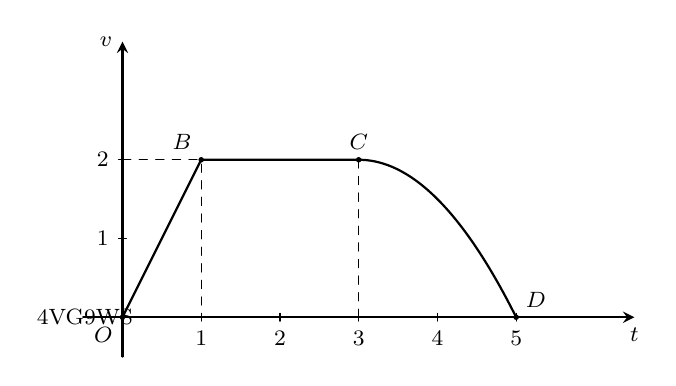
\begin{tikzpicture}[scale=1, line join=round, line cap=round, >=stealth, font=\footnotesize]
    %hidden: VM005
			%			\draw[gray!50, dashed, step=1] (-0.5,-0.5) grid (6.5,3.5);
			\draw[->, thick] (-0.5,0) -- (6.5,0) node[below] {$t$};
			\draw[->, thick] (0,-0.5) -- (0,3.5) node[left] {$v$};
			\foreach \x in {1,2,3,4,5} \draw (\x,0.05) -- (\x,-0.05) node[below] {$\x$};
			\foreach \y in {1,2} \draw (0.05,\y) -- (-0.05,\y) node[left] {$\y$};
			\coordinate (O) at (0,0);
			\coordinate (B) at (1,2);
			\coordinate (C) at (3,2);
			\coordinate (D) at (5,0);
			\fill (O) circle (1pt) node[below left] {$O$};
			\fill (B) circle (1pt) node[above left] {$B$};
			\fill (C) circle (1pt) node[above] {$C$};
			\fill (D) circle (1pt) node[above right] {$D$};
			\draw[thick] (O) -- (B) -- (C);
			\draw[thick, domain=3:5, samples=100] plot (\x, {-0.5*(\x-3)^2 + 2});
			\draw[dashed] (0,2)--(B)--(1,0) (C)--(3,0);
    \node at (0,0){\href{4VG9WS}{\tiny \phantom{4VG9WS}}};
		\end{tikzpicture}
	\end{center}
	\choiceTF
		{\True Trong một giây đầu tiên, vận tốc của chất điểm là $v(t)=2t$, $0 \le t \le 1$}
		{\True Quãng đường chất điểm đi được trong hai giây đầu tiên là $3$ (m)}
		{Giá trị của $a$ là $a=-\dfrac{5}{2}$}
		{Quãng đường chất điểm đi được trong khoảng thời gian $4$ giây đầu tiên là $7{,}7$ (m) (làm tròn đến hàng phần mười)}
	\loigiai{
		\begin{itemchoice}
			\itemch Trong $1$ giây đầu tiên, đồ thị hàm số $v(t)$ là đoạn thẳng $OB$ đi qua gốc tọa độ $O(0;0)$ và điểm $B(1;2)$.\\
			Đường thẳng $OB$ có phương trình dạng $v(t) = kt$, $k$ là hằng số.\\
			Thay tọa độ $B(1;2)$ vào ta được $2 = k \cdot 1 \Rightarrow k = 2$.\\
			Vậy $v(t) = 2t$ với $0 \le t \le 1$.
			\itemch Quãng đường chất điểm đi được trong $2$ giây đầu tiên là
			\[s= \displaystyle\int\limits_0^2 v(t) \mathrm{\, d}t = \displaystyle\int\limits_0^1 (2t) \mathrm{\, d}t +\displaystyle\int\limits_1^2 2 \mathrm{\, d}t=1+2=3.\]	
			\itemch	Trên đoạn $[3;5]$, đồ thị là một phần của parabol có đỉnh $C(3;2)$ nên phương trình có dạng $v(t) = a(t-3)^2 + 2.$\\
			Đồ thị parabol đi qua điểm $D(5;0)$ nên $$0 = a(5-3)^2 + 2 \Leftrightarrow 4a = -2 \Leftrightarrow a = -\dfrac{1}{2}.$$
			\itemch Quãng đường chất điểm đi được trong $4$ giây đầu tiên là
			\[S_4 = \displaystyle\int\limits_0^4 v(t) \mathrm{\, d}t = \displaystyle\int\limits_0^1 2t \mathrm{\, d}t + \displaystyle\int\limits_1^3 2 \mathrm{\, d}t + \displaystyle\int\limits_3^4 \left[ -\dfrac{1}{2}(t-3)^2 + 2 \right] \mathrm{d}t.\]
			Ta có
			\begin{itemize}
				\item $\displaystyle\int\limits_0^1 2t \mathrm{\, d}t = 1$\, (m).
				\item $\displaystyle\int\limits_1^3 2 \mathrm{\, d}t = 2 \cdot 2 = 4$ (m).
				\item $\displaystyle\int\limits_3^4 \left[ -\dfrac{1}{2}(t-3)^2 + 2 \right] \mathrm{d}t = \left[ -\dfrac{1}{6}(t-3)^3 + 2t \right]_{3}^{4} = \left(-\dfrac{1}{6} + 8\right) - 6 = \dfrac{11}{6}$ (m).
			\end{itemize}			
			Vậy $S_4 = 1 + 4 + \dfrac{11}{6} = \dfrac{41}{6} \approx 6{,}8$ (m). 
		\end{itemchoice}
	}
\end{ex}

\Closesolutionfile{ans}
\caukq
\Opensolutionfile{ans}[ans/ans\currfilebase-Phan-III]
\begin{ex}%[Dự án 1YLKNH-VN-MT-15]%[2-KS-21-SoSonLa-L2-2026,VM028]%[2D1V3-6]
	Trong kế hoạch khai thác tuyến ca nô cao tốc phục vụ du lịch sinh thái trên vùng lòng hồ Thủy điện Sơn La (từ bến Mường La đi Quỳnh Nhai) có chiều dài $100$\,km. Ban quản lý cần xác định vận tốc khai thác $v$ (km/h) cho ca nô ($30 \le v \le 70$) để đạt lợi nhuận kinh tế cao nhất. Các dữ kiện của bài toán được xác định như sau: công suất tiêu thụ điện của động cơ ca nô là $P(v)=10v^3$ (W); giá điện kinh doanh tại bến sạc là $2\,000$ đồng/kWh; chi phí vận hành cố định bao gồm nhân lực lái tàu, khấu hao và bến bãi là $2\,500\,000$ đồng cho mỗi giờ ca nô chạy; số lượng khách mua vé cho mỗi chuyến phụ thuộc vào vận tốc khai thác theo hàm số $N(v)=\dfrac{v}{5}+20$ (hành khách); giá vé bình quân cho tuyến này là $500\,000$ đồng/khách. Biết rằng điện năng tiêu thụ của ca nô trong mỗi chuyến là $A=P(v) \cdot t$ (Wh), trong đó $t$ là thời gian ca nô di chuyển hết quãng đường $100$\,km với vận tốc $v$.	Để lợi nhuận ròng (phần tiền còn lại sau khi đã trừ hết mọi chi phí) của mỗi chuyến ca nô trên tuyến này lớn nhất thì vận tốc khai thác $v$ (km/h) bằng bao nhiêu?
	\par
	\shortans{$50$}
	\loigiai{
		Thời gian ca nô chạy hết quãng đường $100$\,km là $t=\dfrac{100}{v}$ (giờ).\\
		Điện năng tiêu thụ cho một chuyến đi là
		\[A=P(v) \cdot t=10v^3 \cdot \dfrac{100}{v}=1\,000v^2 \text{ (Wh)}=v^2 \text{ (kWh)}.
		\]
		Chi phí tiền điện là $C_1(v)=2\,000 \cdot v^2$.\\
		Chi phí vận hành cố định là $C_2(v)=2\,500\,000 \cdot \dfrac{100}{v}=\dfrac{250\,000\,000}{v}$.\\
		Tổng doanh thu từ bán vé là $R(v)=500\,000 \cdot \left(\dfrac{v}{5}+20\right)=100\,000v+10\,000\,000$.\\
		Hàm lợi nhuận ròng của mỗi chuyến là
		\begin{align*}
			L(v)&=R(v)-\big[C_1(v)+C_2(v)\big]\\
			&=-2\,000v^2+100\,000v+10\,000\,000-\dfrac{250\,000\,000}{v} \text{ (đồng)}\\
			&=-2v^2+100v+10\,000-\dfrac{250\,000}{v} \text{ (nghìn đồng)}.
		\end{align*}
		Xét hàm $L(v)$ trên đoạn $[30; 70]$, ta có
		\[L'(v)=-4v+100+\dfrac{250\,000}{v^2}.
		\]
		\begin{eqnarray*}
			L'(v)=0 &\Leftrightarrow &\dfrac{-4v^3+100v^2+250\,000}{v^2}=0\\
			&\Leftrightarrow &v^3-25v^2-62\,500=0\\
			&\Leftrightarrow &(v-50)(v^2+25v+1\,250)=0\\
			&\Leftrightarrow &\hoac{&v=50\\&v^2+25v+1\,250=0 \text{ (vô nghiệm)}.}
		\end{eqnarray*}
		Ta có
		\begin{itemize}
			\item $L(30)=-2\cdot 30^2+100\cdot30+10\,000-\dfrac{250\,000}{30} \approx 2\,866{,}667$.
			\item $L(50)=-2\cdot 50^2+100\cdot50+10\,000-\dfrac{250\,000}{50}=5\,000$.
			\item $L(70)=-2\cdot 70^2+100\cdot70+10\,000-\dfrac{250\,000}{70} \approx 3\,628{,}571$.
		\end{itemize}
		Suy ra $\max\limits_{[30;70]}L(v)=5\,000$ (nghìn đồng).\\
		Vậy lợi nhuận ròng lớn nhất (bằng $5$ triệu đồng) khi vận tốc khai thác là $v=50$ (km/h).
	}
\end{ex}

\begin{ex}%[Dự án 4DUOJZ-VN-MT-15]%[2-KS-21-SoSonLa-L2-2026,VM028]%[2D4V3-2]
	Một xưởng mộc tại Mai Sơn sản xuất những chiếc bàn cờ Ô ăn quan bằng gỗ nguyên khối. Mặt trên của bàn cờ là một mặt phẳng được thiết kế và có kích thước như hình vẽ gồm ba phần: phần chính giữa là một hình chữ nhật có chiều dài $100$\,cm và chiều rộng $40$\,cm; hai "ô quan" ở hai đầu trái và phải là hai hình phẳng bằng nhau được ghép nối liền mạch với hai cạnh chiều rộng của hình chữ nhật. Biết rằng đường bao ngoài của mỗi "ô quan" là một cung tròn. Xưởng mộc tiến hành phủ một lớp keo bảo vệ bóng lên toàn bộ bề mặt trên của chiếc bàn cờ này. Biết chi phí vật tư và nhân công để phủ keo là $100\,000$ đồng/m$^2$. Tổng chi phí $x$ (nghìn đồng) để hoàn thiện việc phủ keo cho mặt bàn cờ bằng bao nhiêu \textit{(làm tròn kết quả đến hàng đơn vị)}?
	\begin{center}
		\begin{tikzpicture}[scale=0.8,line cap=round,line join=round,font=\footnotesize,>=stealth,x=0.1cm,y=0.1cm]
    %hidden: VM005
			\draw (0,0) rectangle (100,40);
			\foreach \x in {20,40,60,80} \draw (\x,0)--(\x,40);
			\draw (0,20)--(100,20);
			\draw (100,40) arc (53.13:-53.13:25);
			\draw (0,0) arc (233.13:126.87:25);
			\draw[<->] (0,50)--(100,50) node[midway, fill=white, inner sep=1.5pt] {$100$\,cm};
			\draw[dashed] (0,42)--(0,52) (100,42)--(100,52);
			\draw[<->] (120,0)--(120,40) node[midway, fill=white, inner sep=1.5pt,rotate=-90] {$40$\,cm};
			\draw[dashed] (103,0)--(123,0) (103,40)--(123,40);
			\draw[<->] (100,-7)--(110,-7) node[midway, below] {$10$\,cm};
			\draw[dashed] (110,14)--(110,-8) (100,-2)--(100,-8);
    \node at (0,0){\href{4DUOJZ}{\tiny \phantom{4DUOJZ}}};
		\end{tikzpicture}
	\end{center}
	\par
	\shortans{$46$}
	\loigiai{
		\begin{center}
			\begin{tikzpicture}[scale=1,line cap=round,line join=round,font=\footnotesize,>=stealth,x=0.08cm,y=0.08cm]
    %hidden: VM005
				\draw (0,0) rectangle (100,40);
				\foreach \x in {20,40,60,80} \draw (\x,0)--(\x,40);
				\draw (0,20)--(100,20);
				\draw (100,40) arc (53.13:-53.13:25);
				\draw (0,0) arc (233.13:126.87:25);
				\draw[<->] (0,50)--(100,50) node[midway, fill=white, inner sep=1.5pt] {$100$\,cm};
				\draw[dashed] (0,42)--(0,52) (100,42)--(100,52);
				\draw[<->] (120,0)--(120,40) node[midway, fill=white, inner sep=1.5pt,rotate=-90] {$40$\,cm};
				\draw[dashed] (103,0)--(123,0) (103,40)--(123,40);
				\draw[<->] (100,-7)--(110,-7) node[midway, below] {$10$\,cm};
				\draw[dashed] (110,14)--(110,-8) (100,-2)--(100,-8);
				\node at (50,-20){Hình $1$};
    \node at (0,0){\href{4DUOJZ}{\tiny \phantom{4DUOJZ}}};
			\end{tikzpicture}
			\qquad		\qquad
			\begin{tikzpicture}[scale=1,line cap=round,line join=round,font=\footnotesize,>=stealth,x=0.08cm,y=0.08cm]
    %hidden: VM005
				\def\R{25}
				\pgfmathsetmacro{\a}{atan(20/15)}
				\path
					coordinate (O) at (15,15)
					coordinate (I) at (30,15)
					coordinate (M) at (40,15)
					coordinate (A) at (30,-5)
					coordinate (B) at (30,35);
				\draw (O)--(M) (A)--(B)--(O)--cycle;
				\draw (O)++(-\a:\R) arc (-\a:\a:\R);
				\draw [dashed] (O)++(\a:\R) arc (\a:360-\a:\R);
				\foreach \P/\p in {A/-60, B/60, O/180, I/-60, M/0}
				\fill (\P) circle (1pt) node at ($(\P)+(\p:3)$) {$\P$};
				\pic[draw, angle radius=2mm] {right angle=O--I--B};
				\pic[draw, angle radius=3mm, "$\alpha$", angle eccentricity=1.7] {angle=M--O--B};
				\node at ($(O)!0.5!(B)+(-2,2)$){$R$};
				\node at (15,-20){Hình $2$};
    \node at (0,0){\href{4DUOJZ}{\tiny \phantom{4DUOJZ}}};
			\end{tikzpicture}
		\end{center}
		Mặt bàn cờ gồm một hình chữ nhật ở chính giữa và hai "ô quan" nằm tại hai đầu. Mỗi ô quan là một hình viên phân được giới hạn bởi một cung tròn và dây cung tương ứng, trong đó dây cung có độ dài $40$\,cm và chiều cao của hình viên phân là $10$\,cm (xem hình $1$).\\
		Hình chữ nhật có diện tích là $S_1=100 \cdot 40=4\,000$ (cm$^2$).\\
		Xét hình tròn tâm $O$ bán kính $R$ với dây cung $AB=40$. Gọi $I$ là trung điểm của $AB$ và $M$ là điểm chính giữa cung nhỏ $\wideparen{AB}$ thì $IM=10$ (xem hình $2$).\\
		Trong $\triangle OBI$ vuông tại $I$ ta có
		\[OB^2=IB^2+OI^2 \Rightarrow R^2=20^2+(R-10)^2 \Rightarrow R=25.
		\]
		Gọi $\alpha=\widehat {BOM}$ (đơn vị Radian), ta có $\sin\alpha=\dfrac{IB}{OB}=\dfrac{20}{25}=0{,}8$.\\
		Hình quạt tròn $OAB$ có số đo là $2\alpha$ và bán kính $R=25$ nên có diện tích là
		\[ S_{\text{quạt}}=\dfrac{2\alpha}{2\pi}\cdot\pi R^2=\alpha\cdot 25^2=625\alpha.
		\]
		$\triangle OAB$ với chiều cao $OI=25-10=15$ có diện tích là
		\[ S_{\triangle OAB}=\dfrac{1}{2} \cdot AB \cdot OI=\dfrac{1}{2} \cdot 40 \cdot 15=300. \]
		Diện tích hình viên phân là
		\[ S_{vp}=S_{\text{quạt}}-S_{\triangle OAB}=625\alpha-300.\]
		Tổng diện tích bề mặt cần phủ keo là
		\[S=S_1+2S_{vp}=4\,000+2(625\alpha-300)=3\,400+1\,250\alpha.
		\]
		Vì chi phí phủ keo là $100\,000$ đồng/m$^2$, tức là $10$ đồng/cm$^2$ nên tổng chi phí phủ keo là
		\[C=S \cdot 10=(3\,400+1\,250\alpha)\cdot 10=34\,000+12\,500\alpha \text{ (đồng)}=34+12{,}5\alpha \text{ (nghìn đồng)}.
		\]
		Do $\sin\alpha=0{,}8\Rightarrow \alpha \approx 0{,}927$ nên $C\approx46$ (nghìn đồng).\\
		Vậy $x=46$.\\
		\textit{Cách khác:} Để tính diện tích hình viên phân ta có thể sử dụng tích phân như sau:\\
		Từ $\triangle OBI$ vuông tại $I$, $R=OM=25$, $OI=15$ ta chọn hệ trục tọa độ $Oxy$ với gốc $O(0;0)$ là tâm đường tròn, trục $Ox$ đi qua trung điểm $I$ của dây cung $AB$ (xem hình dưới đây). 
		\begin{center}
			\begin{tikzpicture}[scale=1,line cap=round,line join=round,font=\footnotesize,>=stealth,x=0.08cm,y=0.08cm]
    %hidden: VM005
				\def\R{25}
				\pgfmathsetmacro{\a}{atan(20/15)}
				\draw[->] (-5-25,0)--(35,0) node[below] {$x$};
				\draw[->] (0,-25-5)--(0,25+5) node[left] {$y$};
				\path
					(0,0) coordinate (O)
					(15,0) coordinate (I)
					(25,0) coordinate (M)
					(15,-20) coordinate (A)
					(15,20) coordinate (B);
				\draw[fill=gray!20,draw=none] (15,-20)--(15,20) arc (\a:-\a:\R)--cycle;
				\draw (A)--(B)--(O)--cycle (O) circle (\R);
				\draw[dashed] (I)--(M);
				\node at ($(O)!0.5!(B)+(-2,2)$){$R$};
				\foreach \P/\p in {O/225, A/-45, B/45, I/-120, M/-45}
				\fill (\P) circle (1pt) node at ($(\P)+(\p:3.5)$) {$\P$};
				\pic[draw, angle radius=2mm] {right angle=O--I--B};
				\pic[draw, "$\alpha$", angle eccentricity=1.7, angle radius=3mm] {angle=I--O--B};
    \node at (0,0){\href{4DUOJZ}{\tiny \phantom{4DUOJZ}}};
			\end{tikzpicture}
		\end{center}
		Khi đó\\
		Phương trình đường tròn $x^2+y^2=25^2 \Rightarrow y=\pm \sqrt{625-x^2}$.\\
		Tọa độ các điểm $I(15;0)$, $M(25;0)$, dây cung $AB$ nằm trên đường thẳng $x=15$.\\
		Hình viên phân giới hạn bởi cung tròn $AMB$ và đoạn thẳng $AB$ có diện tích là
		\[S_{vp}=2 \displaystyle\int\limits_{15}^{25} \sqrt{625-x^2}\mathrm{\,d}x.
		\]
		Sử dụng máy tính cầm tay, tính được $S_{vp} \approx279{,}56$ (cm$^2$).
	}
\end{ex}

\begin{ex}%[Dự án 3L9CTI-VN-MT-15]%[2-KS-21-SoSonLa-L2-2026,VM028]%[1D2V3-8]
	Một cá nhân gây thiệt hại cho tài sản nhà nước với tổng số tiền là $450$ triệu đồng. Để được giảm nhẹ trách nhiệm hình sự, người này được yêu cầu phải hoàn thành việc bồi thường ít nhất $60\%$ tổng số tiền gốc trong vòng $6$ tháng đầu tiên. Phương thức bồi thường được thỏa thuận như sau: Tháng thứ nhất người đó nộp $m$ (triệu đồng); kể từ tháng thứ hai, mỗi tháng số tiền nộp bằng $90\%$ số tiền đã nộp ở tháng liền trước đó. Để được giảm nhẹ trách nhiệm hình sự, người này phải nộp tháng đầu tiên với số tiền $m$ nhỏ nhất là bao nhiêu \textit{(không làm tròn kết quả các phép tính trung gian, chỉ làm tròn kết quả cuối cùng đến hàng đơn vị)}?
	\par
	\shortans{$58$}
	\loigiai{
		Số tiền người đó cần phải bồi thường trong $6$ tháng đầu tiên là
		\[450 \cdot 60\%=270 \text{ (triệu đồng).}
		\]
		Tháng thứ nhất người đó nộp $m$ (triệu đồng).\\
		Vì kể từ tháng thứ hai, mỗi tháng số tiền nộp bằng $90\%$ số tiền đã nộp ở tháng liền trước đó nên số tiền nộp mỗi tháng lập thành một cấp số nhân có số hạng đầu là $u_1=m$ và công bội $q=90\%=0{,}9$.\\
		Tổng số tiền nộp sau $6$ tháng là tổng của $6$ số hạng đầu của cấp số nhân
		\[S_6=u_1 \cdot \dfrac{1-q^6}{1-q}=m \cdot \dfrac{1-(0{,}9)^6}{1-0{,}9}=m \cdot 4{,}68559.
		\]
		Để được giảm nhẹ trách nhiệm hình sự thì phải có
		\[S_6 \ge 270 \Leftrightarrow m \cdot 4{,}68559 \ge 270 \Leftrightarrow m \ge \dfrac{270}{4{,}68559} \approx 57{,}6235.
		\]
		Vì $m$ là số tiền nộp và đề bài yêu cầu làm tròn đến hàng đơn vị, đồng thời $m$ phải thỏa mãn điều kiện bồi thường ít nhất $60\%$, nên ta chọn giá trị nguyên nhỏ nhất thỏa mãn điều kiện trên là $m=58$.\\
		Vậy số tiền $m$ nhỏ nhất nộp trong tháng đầu tiên là $58$ triệu đồng.
	}
\end{ex}

\begin{ex}%[Dự án 50XS9J-VN-MT-15]%[2-KS-21-SoSonLa-L2-2026,VM026]%[1H8V5-4]
	Cho hình chóp $S.ABCD$ có đáy là hình thang, $AB = 2a$, $AD = DC = CB = a$, $SA$ vuông góc với mặt phẳng đáy và $SA = 3a$. Gọi $M$ là trung điểm của $AB$. Khoảng cách giữa hai đường thẳng $SB$ và $DM$ bằng $\dfrac{xa}{y}$ (với $x$, $y \in \mathbb{N}^*$, $\dfrac{x}{y}$ tối giản). Giá trị của $T = x + y + xy$  bằng bao nhiêu?
	\begin{center}
		\begin{tikzpicture}[scale=1, font=\footnotesize, line join=round, line cap=round, >=stealth]
    %hidden: VM005
			\def\a{5}
			\def\h{4}
			\path 	(0:0) coordinate (A)
				++(0:\a) coordinate (B)
				($(A)+(-120:\a/2)$) coordinate (D)
				($(B)+(D)-(A)$) coordinate (Ct)
				($(D)!1/2!(Ct)$) coordinate (C)
				($(A)+(90:\h)$) coordinate (S)
				($(A)!0.5!(B)$) coordinate (M)
				($(S)!0.6!(C)$) coordinate (H)
				(intersection of A--C and B--D) coordinate (O);%giao điểm O
			\draw[dashed] 	(B)--(A)--(D)--(M)--(C)	(A)--(S) (C)--(A)--(H);
			\draw 			(B)--(C)--(D)
				(B)--(S)	(C)--(S)	(D)--(S);
			\foreach \x/\g in {A/135,B/45,C/-45,D/-135,S/90, M/90, H/30}
			\fill (\x) circle (1pt)
				($(\g:3mm)+(\x)$) node {$\x$};	
			\draw pic[draw,angle radius=2mm]{right angle=B--A--S};
			\draw pic[draw,angle radius=2mm]{right angle=S--H--A};
    \node at (0,0){\href{50XS9J}{\tiny \phantom{50XS9J}}};
		\end{tikzpicture}	
	\end{center}
	\par
	\shortans{$19$}
	\loigiai{
		Vì $M$ là trung điểm của $AB$ nên $AM = MB = \dfrac{1}{2}AB = a$.\\
		Tứ giác $AMCD$ có $AM \parallel DC$ ($AB \parallel DC$) và $AM = DC = a$ nên $AMCD$ là hình bình hành.\\
		Lại có $AD = AM = a$ nên $AMCD$ là hình thoi. Suy ra $CM = a$.\\
		Trong tam giác $ABC$ có trung tuyến $CM = \dfrac{1}{2}AB = a$, do đó tam giác $ABC$ vuông tại $C$, hay $AC \perp BC$.\\
		Mặt khác, xét tứ giác $MBCD$ có $MB \parallel DC$ và $MB = DC = a$ nên $MBCD$ là hình bình hành.\\
		Suy ra $DM \parallel BC$. Mà $BC \subset (SBC)$ nên $DM \parallel (SBC)$.\\
		Khi đó $\mathrm{d}(DM, SB) = \mathrm{d}\big(DM, (SBC)\big) = \mathrm{d}\big(M, (SBC)\big)$.\\
		Vì $AB \cap (SBC) = B$ và $M$ là trung điểm $AB$ nên $\mathrm{d}\big(M, (SBC)\big) = \dfrac{1}{2}\mathrm{d}\big(A, (SBC)\big)$.\\		
		Ta có $\heva{&BC \perp AC \\ &BC \perp SA ~\text{(do } SA \perp (ABCD)\text{)}} \Rightarrow BC \perp (SAC)$.\\
		Kẻ $AH \perp SC$ ($H \in SC$). Vì $BC \perp (SAC) \Rightarrow BC \perp AH$.\\
		Suy ra $AH \perp (SBC) \Rightarrow \mathrm{d}\big(A, (SBC)\big) = AH$.\\
		Trong tam giác vuông $ABC$ có $AC = \sqrt{AB^2 - BC^2} = \sqrt{(2a)^2 - a^2} = a\sqrt{3}$.\\
		Trong tam giác vuông $SAC$ có  
		\[ \dfrac{1}{AH^2} = \dfrac{1}{SA^2} + \dfrac{1}{AC^2} = \dfrac{1}{(3a)^2} + \dfrac{1}{(a\sqrt{3})^2} = \dfrac{1}{9a^2} + \dfrac{1}{3a^2} = \dfrac{4}{9a^2} \Rightarrow AH = \dfrac{3a}{2}. \]
		Vậy $\mathrm{d}(DM, SB) = \dfrac{1}{2} \cdot \dfrac{3a}{2} = \dfrac{3a}{4}$.\\
		Đối chiếu $\mathrm{d} = \dfrac{xa}{y}$ ta được $x = 3$, $y = 4$ (thỏa mãn $\dfrac{3}{4}$ tối giản).\\
		Giá trị $T = x + y + xy = 3 + 4 + 3 \cdot 4 = 19$.
	}
\end{ex}

\begin{ex}%[Dự án 5NIPB6-VN-MT-15]%[2-KS-21-SoSonLa-L2-2026,VM026]%[0D0C2-9]
	Trong một trò chơi thám hiểm, anh Sơn phải vượt qua một mê cung gồm các phòng thông nhau như sơ đồ dưới đây. Tại mỗi phòng, anh Sơn sẽ chọn ngẫu nhiên một trong các cửa thông với phòng hiện tại (với xác suất như nhau) để đi tiếp. Quá trình di chuyển diễn ra liên tục và trò chơi sẽ kết thúc ngay khi anh bước vào phòng chứa Kho báu hoặc phòng có Bẫy. Biết anh Sơn bắt đầu từ Phòng 1, xác suất để anh tìm được kho báu bằng bao nhiêu (kết quả làm tròn đến hàng phần trăm)?
	\begin{center}
		\begin{tikzpicture}[scale=1, line join=round, line cap=round, transform shape]
    %hidden: VM005
			% --- ĐỊNH NGHĨA MÀU ---
			\definecolor{wood}{HTML}{5D2906}
			\definecolor{gold}{HTML}{FFD700}
			\definecolor{sand}{HTML}{C2B280}
			\def\w{3}
			\def\h{2.5}
			\tikzset{ruong/.pic = {
			\def\g{-130}
			\path (0,0) coordinate (A)
				(\g:2) coordinate (B)
				++(0:4) coordinate (C)
				($(A)+(C)-(B)$) coordinate(D);
			\foreach \i in {A,B,C,D} \path ($(\i)+(90:2.3)$) coordinate(\i');
			\path (D')--++(120:2) coordinate(E) --++(-4,0) coordinate(F);
			\fill[draw, wood!70] (A)--(B)--(B')--(A') (A)--(D)--(D')--(A');
			\draw[wood] (A)--(A');
			\fill[line width=2pt,draw=wood, fill=wood!50] (A')--(B')--(B)--(C)--(D)--(D')--(C')--(B') (A')--(D') (C)--(C');
			\def\NP{(E) .. controls ++(25:0.7) and ++(80:1.5) .. (D') coordinate[pos=0.19](e)}
			\def\NT{(F) .. controls ++(25:0.7) and ++(80:1.5) .. (A')coordinate[pos=0.19](f)};
			\fill[draw, top color=wood!90, middle color=wood!80, bottom color=wood!50] (E)--(F)--\NT -- (D') ..controls ++(80:1.5) and ++(25:0.7) .. (E);
			\fill[draw=wood, fill=gold] (D')--\NP;
			\fill[draw=wood, fill=wood!95] (D')++(105:0.3) coordinate(d') --++(120:1.55) .. controls ++ (25:0.5) and ++(80:1) .. (d');
			\fill[draw=wood, fill=wood!95] (A')--\NT;	
			\fill[draw=wood,wood] ($(A')+(180:1pt)$) -- ++(120:2)--++(0:2pt)--++(-60:2)--cycle ($(D')+(180:2pt)$) -- ++(120:2)--++(0:2pt)--(D')--cycle
				($(E)+(180:2pt)$)--++(180:3.9)--++(-60:2pt)--++(0:3.9)--cycle
				($(D')+(180:2pt)$)--++(180:3.97)--++(-60:2pt)--++(0:3.97)--cycle;
			\fill[draw=gold, gold] (E) .. controls ++(25:0.15)..(e)--(f)..controls ++(170:0.2) and +(70:0.05)..($(F)+(180:1pt)$)--(E);
			\shade[left color=gold!60!brown, right color=gold, middle color=gold!70!white] ($(B)+(-1pt,-1pt)$)--($(C)+(1pt,-1pt)$)--($(C')+(1pt,-1pt)$)--($(B')+(-1pt,-1pt)$)--cycle;
			\shade[left color=gold!40!brown, right color=gold, middle color=gold!70!white] ($(C)+(1pt,-1pt)$)--($(C')+(1pt,-1pt)$)--($(D')+(1pt,-1pt)$)--($(D)+(1pt,-1pt)$)--cycle;
			\fill[wood, rounded corners] ($(B)+(0.24,0.24)$) coordinate(l1) rectangle ++(0.76,1.8) ($(B)+(1.25,0.24)$) coordinate(l2) rectangle ++(1.5,1.8) ($(C)+(-0.24,0.24)$) coordinate(l3) rectangle ++(-0.76,1.8)
				($(C)+(50:0.28)$)++(90:0.24) coordinate(r) --++(50:1.5)--++(90:1.8)--++(\g:1.5)--cycle;
			\begin{scope}
				\clip[rounded corners] (l1) rectangle ++(0.76,1.8);
				\foreach \i in {1,2,3} {\draw[thick, wood!50!black] ($(l1)+(90:0.45*\i)$) --++(0:0.75);}
				\draw[wood!50!black, thick, rounded corners] (l1)--++(90:1.8)--++(0:0.74);
			\end{scope}
			\begin{scope}
				\clip[rounded corners] (l2) rectangle ++(1.5,1.8);
				\foreach \i in {1,2,3} {\draw[thick, wood!50!black] ($(l2)+(90:0.45*\i)$) --++(0:2);}
				\draw[wood!50!black, thick, rounded corners] (l2)--++(90:1.8)--++(0:2);
			\end{scope}
			\begin{scope}
				\clip[rounded corners] (l3) rectangle ++(-0.76,1.8);
				\foreach \i in {1,2,3} {\draw[thick, wood!50!black] ($(l3)+(90:0.45*\i)$) --++(180:1);}
				\draw[wood!50!black, thick, rounded corners] (l3)++(180:0.76)--++(90:1.8)--++(0:1);
			\end{scope}
			\begin{scope}
				\clip[rounded corners] (r) --++(50:1.5)--++(90:1.8)--++(\g:1.5)--cycle;
				\foreach \i in {1,2,3} {\draw[thick, wood!50!black] ($(r)+(90:0.45*\i)$) --++(50:2);}
				\draw[wood!50!black, thick, rounded corners] (r)--++(50:1.5)--++(90:1.8);
			\end{scope}
			\begin{scope}
				\clip (A')--(B')--(C')--(D')--(A');
				\foreach \i in {1,...,500} {
				\shade[ball color=gold] ({random(-10,45)/10}, {random(9,21)/10}) ellipse (0.2 and 0.14);
				}
			\end{scope}
			\fill[draw=gold!80!black, fill=gold, rounded corners] ($(B')!0.43!(C')$)++(-90:0.15) coordinate(k1) rectangle ++(0.6,-0.6);
			\fill (k1)++(0.25,-0.3) arc(-120:300:{0.1}) --++(-90:0.22)--++(180:0.1)--cycle;
			\fill[draw=gold!80!black, fill=gold, rounded corners=0.01] ($(F)!0.43!(E)$) coordinate(k2)--++(\g:0.5)--++(0:0.5)--++(50:0.5)--cycle;
			\fill[black,rotate=-50] (k2)++(0.2,-0.1) ellipse(0.08 and 0.12);}}
			% --- 1. VẼ TƯỜNG MÊ CUNG ---
			% Hàng 1
			\draw (0,\h) -- (0,2*\h) -- (3*\w,2*\h) -- (3*\w,\h);
			% Hàng 2
			\draw (1*\w,0) -- (3*\w,0);
			\draw (3*\w,0) rectangle (4*\w,\h);
			% Các vách ngăn dọc
			\draw (0, \h) -- (1.5*\w, \h); 
			\draw (1.7*\w, \h) -- (3*\w, \h);
			\draw (1*\w, 0) -- (1*\w, 2*\h);
			\draw (2*\w, 0) -- (2*\w, 2*\h); 
			% --- 2. VẼ CỬA THÔNG (Đè đường trắng) ---
			\begin{scope}[white, line width=4pt]
				\draw (\w, 1.3*\h) -- (\w, 1.7*\h); 
				\draw (2*\w, 1.3*\h) -- (2*\w, 1.7*\h); 
				\draw (1.3*\w, \h) -- (1.7*\w, \h); 
				\draw (2.3*\w, \h) -- (2.7*\w, \h); 
				\draw (2*\w, 0.3*\h) -- (2*\w, 0.7*\h); 
				\draw (3*\w, 0.3*\h) -- (3*\w, 0.7*\h); 
			\end{scope}
			% --- 3. CHÈN HÌNH MINH HỌA CHI TIẾT ---	
			% A. CHÈN RƯƠNG KHO BÁU (Tại tọa độ Kho báu)
			\begin{scope}[shift={(0.4*\w, 1.6*\h)}]
				\path (0,0) pic[scale=0.2]{ruong};
			\end{scope}
			% B. CHÈN CẠM BẪY (Tại tọa độ Bẫy)
			\begin{scope}[shift={(3.5*\w, 0.5*\h)}, scale=0.5]
				% Hố chông
				\fill[black!80] (-1,-0.5) rectangle (1,0.5);
				% Chông nhọn
				\foreach \x in {-0.8,-0.4,0,0.4,0.8}
				\fill[gray!60, draw=black, line width=0.2pt] (\x,-0.3) -- (\x-0.15,-0.8) -- (\x+0.15,-0.8) -- cycle;
				\foreach \x in {-0.6,-0.2,0.2,0.6}
				\fill[gray!40, draw=black, line width=0.2pt] (\x,0.1) -- (\x-0.15,-0.4) -- (\x+0.15,-0.4) -- cycle;
				% Biển cảnh báo
				\draw[red, line width=1pt] (0,0.8) -- (-0.6,0) -- (0.6,0) -- cycle;
				\node[red, scale=0.8, font=\boldmath] at (0,0.3) {!};
			\end{scope}
			% --- 4. THÊM VĂN BẢN NHÃN ---
			\node[below] at (0.5*\w, 1.4*\h) {\textbf{Kho báu}};
			\node at (1.5*\w, 1.5*\h) {Phòng 1};
			\node at (2.5*\w, 1.5*\h) {Phòng 2};
			\node at (1.5*\w, 0.5*\h) {Phòng 3};
			\node at (2.5*\w, 0.5*\h) {Phòng 4};
			\node[below] at (3.5*\w, 0.35*\h) {\textbf{Bẫy}};
    \node at (0,0){\href{5NIPB6}{\tiny \phantom{5NIPB6}}};
		\end{tikzpicture}
	\end{center}
	\par
	\shortans{$0{,}67$}
	\loigiai{
		Gọi $P_i$ là xác suất để anh Sơn tìm được kho báu nếu đang đứng ở Phòng $i$ ($i=1, 2, 3, 4$). 
		Dựa vào sơ đồ kết nối và quy tắc chọn cửa ngẫu nhiên, ta có hệ phương trình sau:
		\begin{itemize}
			\item Tại Phòng 1 có $3$ cửa (Kho báu, Phòng 2, Phòng 3):
			\[ P_1 = \dfrac{1}{3} \cdot 1 + \dfrac{1}{3} P_2 + \dfrac{1}{3} P_3. \tag*{$(1)$} \]
			\item Tại Phòng 2 có $2$ cửa (Phòng 1, Phòng 4):
			\[ P_2 = \dfrac{1}{2} P_1 + \dfrac{1}{2} P_4. \tag*{$(2)$} \]
			\item Tại Phòng 3 có $2$ cửa (Phòng 1, Phòng 4):
			\[ P_3 = \dfrac{1}{2} P_1 + \dfrac{1}{2} P_4. \quad \tag*{$(3)$} \]
			\item Tại Phòng 4 có $3$ cửa (Phòng 2, Phòng 3, Bẫy):
			\[ P_4 = \dfrac{1}{3} P_2 + \dfrac{1}{3} P_3 + \dfrac{1}{3} \cdot 0. \tag*{$(4)$} \]
		\end{itemize}
		Từ $(2)$ và $(3)$ ta thấy $P_2 = P_3$. Thay vào $(4)$ ta được
		$P_4 = \dfrac{2}{3} P_2$.\\
		Ta được hệ phương trình
		\[ \heva{& P_1 = \dfrac{1}{3} + \dfrac{2}{3} P_2 \\ & P_2 = \dfrac{1}{2} P_1 + \dfrac{1}{2} \left( \dfrac{2}{3} P_2 \right)} 
		\Leftrightarrow \heva{& 3P_1 - 2P_2 = 1 \\ & \dfrac{2}{3} P_2 = \dfrac{1}{2} P_1} 
		\Leftrightarrow \heva{& 3P_1 - 2P_2 = 1 \\ & P_2 = \dfrac{3}{4} P_1}\Rightarrow P_1 = \dfrac{2}{3}. \]
		Làm tròn đến hàng phần trăm, xác suất để anh Sơn tìm được kho báu là $0{,}67$.
	}
\end{ex}

\begin{ex}%[Dự án 4AVPUP-VN-MT-15]%[2-KS-21-SoSonLa-L2-2026,VM026]%[0D8V2-9]
	Nhân dịp nghỉ lễ 30/4, siêu thị X in ra $100$ phiếu thưởng được đánh số thứ tự từ $1$ đến $100$, mỗi phiếu ghi $1$ số, các phiếu khác nhau ghi số khác nhau. Mỗi khách hàng trong $100$ khách hàng đầu tiên đến siêu thị trong ngày 30/4 sẽ được nhận $1$ phiếu thưởng. Những người được nhận phiếu thưởng có thể tìm thêm $2$ người khác để ghép thành $1$ nhóm có $3$ người. Nếu tổng các số ghi trên $3$ thẻ của $3$ người trong nhóm bằng $100$ thì mỗi người trong nhóm được nhận $50\,000$đ. Siêu thị quy định:
	\begin{enumerate}
		\item Một người có thể ghép vào nhiều nhóm nên có thể nhận thưởng nhiều lần.
		\item Mỗi nhóm $3$ người chỉ được nhận thưởng $1$ lần.
	\end{enumerate}
	Hỏi ban quản lý siêu thị phải chuẩn bị số tiền thưởng lớn nhất là bao nhiêu triệu đồng (kết quả làm tròn đến hàng đơn vị)?	
	\par \shortans{$118$}
	\loigiai{
		\begin{center}
			\begin{tikzpicture}[scale=0.8, font=\footnotesize]
    %hidden: VM005
				% Mô phỏng các phiếu thưởng
				\foreach \i/\val in {1/10, 2/30, 3/60, 4/1, 5/2, 6/97} {
				\node[draw, fill=yellow!15, minimum width=1cm, minimum height=0.6cm, rounded corners=2pt] (c\i) at ({(\i-1)*1.5},0) {\val};
			}
				% Nhóm 1
				\draw[thick, blue!70, dashed] (c1.north) .. controls +(0,0.5) and +(0,0.5) .. (c2.north);
				\draw[thick, blue!70, dashed] (c2.north) .. controls +(0,0.8) and +(0,0.8) .. (c3.north);
				\node[blue!70, above] at (2.2,0.8) {Nhóm A (Tổng = 100)};
				% Nhóm 2
				\draw[thick, orange!80, dotted] (c4.south) .. controls +(0,-0.5) and +(0,-0.5) .. (c5.south);
				\draw[thick, orange!80, dotted] (c5.south) .. controls +(0,-0.8) and +(0,-0.8) .. (c6.south);
				\node[orange!80, below] at (5.2,-0.8) {Nhóm B (Tổng = 100)};
				\node[anchor=west] at (8,0) {$\dots$ tổng cộng $100$ phiếu};
    \node at (0,0){\href{4AVPUP}{\tiny \phantom{4AVPUP}}};
			\end{tikzpicture}
		\end{center}
		Để số tiền thưởng lớn nhất thì cả $100$ phiếu phải được phát ra và mỗi người nhận được phiếu đều tìm được tất cả các bộ ba của mình, tức là tất cả các bộ ba phiếu thỏa mãn yêu cầu bài toán đều được hình thành.\\
		Giả sử số ghi trên phiếu của ba người trong một nhóm là $x$, $y$, $z$. Khi đó $x$, $y$, $z$ là các số tự nhiên đôi một khác nhau và thỏa mãn $x + y + z = 100$.\\
		Trước hết ta cần tìm số nghiệm nguyên dương đôi một khác nhau của phương trình 
		\[ x + y + z = 100.\]
		Để giải bài toán này, ta thực hiện qua các bước sau:
		\begin{itemize}
			\item[B1:] Tìm số nghiệm nguyên dương của phương trình $x + y + z = 100$.\\
			Theo bài toán chia kẹo Euler, số nghiệm nguyên dương của phương trình $x + y + z = 100$ là
			\[ \mathrm{C}_{100-1}^{3-1} = \mathrm{C}_{99}^2 = \dfrac{99 \cdot 98}{2} = 4\,851.\]
			\item[B2:] Loại bỏ các trường hợp có các số bằng nhau.
			\begin{itemize}
				\item Trường hợp $3$ số $x$, $y$, $z$ bằng nhau. Lúc này ta được phương trình $3x = 100$.\\
				Phương trình này không có nghiệm nguyên dương. \\
				Vậy không có bộ nào cả $3$ số bằng nhau.
				\item Trường hợp $2$ số bằng nhau.\\
				Không mất tính tổng quát, giả sử $x = y \neq z$. Khi đó ta được phương trình $2x + z = 100$.\\
				Vì $z \ge 1$ nên $2x < 100 \Rightarrow x < 50$.\\
				Vì $x$ nguyên dương nên $x \in \{1, 2, 3, \dots, 49\}$.\\
				Như vậy có $49$ giá trị của $x$, với mỗi giá trị $x$ có đúng một giá trị $z$. Do đó ta có $49$ bộ $x$, $z$.\\
				Mỗi bộ giá trị $\{x, x, z\}$ có $3$ cách hoán vị ($xxz, xzx, zxx$).\\
				Vậy số nghiệm có ít nhất $2$ số bằng nhau là $49 \cdot 3 = 147$.
			\end{itemize}
		\end{itemize}
		Suy ra số nghiệm nguyên dương đôi một khác nhau của phương trình trên là $4\,851 - 147 = 4\,704$.\\
		Vì mỗi bộ ba số được phát thưởng có tổng cộng $6$ hoán vị tương ứng với $3!=6$ nghiệm của phương trình trên nên số bộ được phát thưởng là $\dfrac{4\,704}{3!} = 784$.\\
		Vậy số tiền thưởng lớn nhất mà siêu thị cần chuẩn bị là
		\[ 784 \cdot 50\,000\cdot 3 = 117\,600\,000 ~\text{(đồng)} \approx 118~\text{(triệu đồng)}.\]
	}
\end{ex}

\Closesolutionfile{ans}
\Closesolutionfile{ansbook}
\begin{indapan}
	{ans/ans\currfilebase}
\end{indapan}